% Versao 1.0 - Helder Oliveira
% Versao 1.1 - Joahannes Costa
% Versao 1.1.1 - Nagib Matni

% Widescreen
%\documentclass[10pt,aspectratio=169]{beamer}
% 4:3
\documentclass[10pt]{beamer}
\usepackage{amsmath,amssymb,amsfonts}
\usepackage[english]{babel}
\usepackage[utf8]{inputenc}
\usepackage{algorithmic}
\usepackage{subfigure}
\usepackage{graphicx}
\usepackage{textcomp}
\usepackage{verbatim}
\usepackage{booktabs}
\usepackage{xcolor}
\usepackage{float}
\usepackage{cite}
\usepackage{flushend}
\usepackage{color}
\usepackage{multicol}
\usepackage[normalem]{ulem}

\newcommand{\blue}[1]{\textcolor{blue}{#1}}
\newcommand{\red}[1]{\textcolor{red}{#1}}
\newcommand{\green}[1]{\textcolor{green}{#1}}
\newcommand{\yellow}[1]{\textcolor{yellow}{#1}}
\newcommand{\magenta}[1]{\textcolor{magenta}{#1}}


%Exibir notas na segunda tela
% \usepackage{pgfpages}
% \setbeameroption{show notes on second screen}

%OBS: se a barra de progresso quebrar, mexer na
% parte "calculate end position" do arquivo beamerouterthemeLRC.sty
% e somar o número no 360 para corrigir.

\makeatletter
\def\beamer@calltheme#1#2#3{%
\def\beamer@themelist{#2}
    \@for\beamer@themename:=\beamer@themelist\do
{\usepackage[{#1}]{\beamer@themelocation/#3\beamer@themename}}}

\def\usefolder#1{
    \def\beamer@themelocation{#1}
}
\def\beamer@themelocation{}

\usefolder{LRCgraphics}
\usetheme{LRC}

% \definecolor{LRCcolorgreen}{RGB}{34,128,34}
% \definecolor{LRCcolorgrey}{RGB}{193,193,193}
\definecolor{LatinComBlue}{RGB}{0, 91, 150}
\definecolor{LatinComgrey}{RGB}{93, 99, 95}

\setbeamercolor{LRC}{fg=LatinComgrey,bg=LatinComBlue}
\setbeamercolor{block title}{bg=LatinComBlue,fg=white}
\setbeamercolor{structure}{fg=black}
\setbeamercolor{normal text}{fg=black,bg=gray!10}

\setbeamertemplate{section in toc}{%
{\color{LatinComBlue}\inserttocsectionnumber.}~\inserttocsection}
\setbeamercolor{subsection in toc}{bg=white,fg=structure}
\setbeamertemplate{subsection in toc}{%
\hspace{1.2em}{\color{LatinComBlue}\rule[0.3ex]{3pt}{3pt}}~\inserttocsubsection\par}

\mode<presentation>
{
	\setbeamertemplate{enumerate items}[circle]
	\setbeamertemplate{itemize item}[square]
% 	\setbeamertemplate{itemize item}{\small\includegraphics[height=1.6ex]{LRCgraphics/Latincommundo}}
	\setbeamertemplate{itemize subitem}[circle]
	\setbeamertemplate{itemize subsubitem}[triangle]
	\setbeamercolor{item projected}{bg=LatinComBlue}
	\setbeamercolor{itemize item}{fg=LatinComBlue}
	\setbeamercolor{itemize subitem}{fg=LatinComBlue}
	\setbeamercolor{itemize subsubitem}{fg=LatinComBlue}
} 

%-------------------------------------------------------
% INCLUDE PACKAGES
%-------------------------------------------------------

\usepackage[utf8]{inputenc}
\usepackage[english]{babel}
\usepackage[T1]{fontenc}
\usepackage{helvet}

\usepackage{graphicx,subfigure}

%-------------------------------------------------------
% DEFFINING AND REDEFINING COMMANDS
%-------------------------------------------------------

% colored hyperlinks
\newcommand{\chref}[2]{
  \href{#1}{{\usebeamercolor[bg]{\theme\LRC}#2}}
}

%-------------------------------------------------------
% INFORMATION IN THE TITLE PAGE
%-------------------------------------------------------

\title[Service Migration for Connected Autonomous Vehicles\hfill a]
{
    \textcolor{LatinComBlue}{\textbf{A Service Migration for Connected Autonomous Vehicles}}
}

\subtitle[~]
{
      %\textbf{Subtítulo do seu trabalho aqui, comente se não tiver}
}

\author[Pacheco et al. 2020]
{\textbf{Lucas Pacheco}, Helder Oliveira, Denis Ros\'ario, Eduardo Cerqueira, Leandro Villas, Torsten Braun}

\institute[]
{   
%    
\includegraphics[scale=0.3]{LRCgraphics/logo-unicamp.eps}\\
    % 
\includegraphics[width=2in]{LRCgraphics/gercomlogo.jpeg}
    % \vfill
    % \textsc{
    %     Federal University of Pará\\
    %     Technology Institute\\\vspace{-0.1cm}
    %     Computer Network Study Group
    % }
    % \vfill
    
\includegraphics[width=2in]{LRCgraphics/gercomlogo.jpeg}\\
}

\date{\sout{Rennes} Internet, \today}

%-------------------------------------------------------
% THE BODY OF THE PRESENTATION
%-------------------------------------------------------

\begin{document}

%-CAPA
{\1
    % \usebackgroundtemplate{\includegraphics[width=\paperwidth]{images/pontanegra.jpg}}
	\begin{frame}[plain,noframenumbering]
		\titlepage
	\end{frame}
}
%-AGENDA
\begin{frame}{Agenda}{}
	\tableofcontents
\end{frame}

%Aparece menu a cada nova seção
\AtBeginSection[]
{
	\begin{frame}<beamer>
		\frametitle{Agenda}
		\tableofcontents[currentsection]
	\end{frame}
}

%-INICIO
\section{Motivation}
\begin{frame}{Motivation}
    \begin{block}{Connected Autonomous Vehicles}
    \begin{itemize}
        \item Modern Transportation will be completely revolutionized b the presence of Autonomous Vehicles.
        \item Autonomous Vehicles, however, are still not ready to be a standalone device, they must be connected at all times to:
        \begin{itemize}
            \item Share context information.
            \item Offload Data processing.
            \item provide in-vehicle services.
        \end{itemize}
        \item Constituting the notion of \textbf{Connected Autonomous Vehicles}.
    \end{itemize}
    \end{block}
\end{frame}

\begin{frame}{Motivation}
    \begin{block}{Edge-enabled Networks}
    \begin{figure}
        \centering
        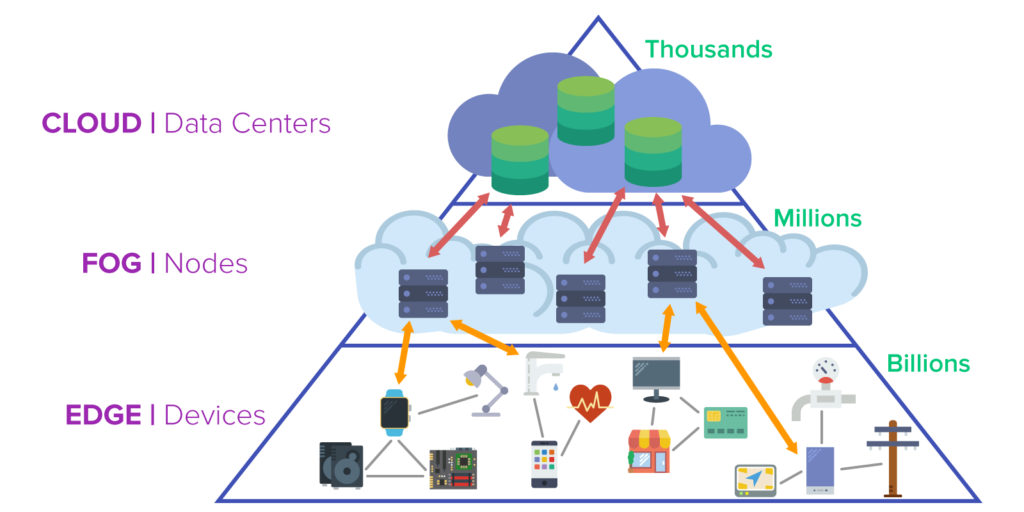
\includegraphics[width=0.7\textwidth]{images/edge_fog.png}
        \caption{Egde-enabled architecture\footnote{https://erpinnews.com/fog-computing-vs-edge-computing}}
        \label{fig:my_label}
    \end{figure}
    \end{block}
\end{frame}

\begin{frame}{Motivation}
    \begin{block}{}
    \end{block}
\end{frame}

\begin{frame}{Motivation}
    \begin{block}{Edge-enabled Networks}
    \begin{itemize}
        \item Edge and Fog computing will be a significant part of 5G and 6G networks.
        \item This aims to bring computing close to end-users reducing latency, and enabling high throughput applications for users.
    \end{itemize}
    \end{block}
\end{frame}

\section{Related Works}

\section{MOSAIC Algorithm}

\section{Experimental Results}

\section{Conclusions}

\begin{frame}{Questions?}
\centering

    \vphantom{1in}
	Find me at:
	
	Email: lucas.pacheco@itec.ufpa.br
	LinkedIn: www.linkedin.com/in/lucas-pacheco-l13
	
	\vfill
	
	\begin{multicols}{3}
\vspace*{\fill}
	\begin{figure}
	    \centering
	    
\includegraphics[width=0.2\textwidth]{images/ppgee.png}
	\end{figure}
\vspace*{\fill}
	\begin{figure}
	    \centering
	    
\includegraphics[width=0.2\textwidth]{images/ufpa.png}
	\end{figure}
	\vspace*{\fill}
	\begin{figure}
	    \centering
	    
\includegraphics[width=0.2\textwidth]{images/capes.png}
	\end{figure}
    \vspace*{\fill}
	\end{multicols}
\end{frame}

\end{document}